% ============================================================================
%  Hippocampus Memory Architecture: From pgvector to Typed Directed Hypergraph
%  Date: March 2026
%  Epistemic Convention:
%    [Verified]             -- Confirmed in codebase or published documents
%    [Synthesized]          -- Derived from multiple verified sources
%    [Speculative Proposal] -- Architectural direction not yet implemented
% ============================================================================

\documentclass[11pt]{article}
\usepackage[margin=1in]{geometry}
\usepackage[T1]{fontenc}
\usepackage[utf8]{inputenc}
\usepackage{amsmath, amssymb, amsthm}
\usepackage{mathtools}
% \usepackage{algorithm}     % not available; replaced with custom tcolorbox
% \usepackage{algpseudocode} % not available; replaced with manual pseudocode
\usepackage{hyperref}
\usepackage{graphicx}
\usepackage{booktabs}
\usepackage{enumitem}
\usepackage{xcolor}
\usepackage{tcolorbox}
\usepackage{tikz}
\usetikzlibrary{arrows.meta, positioning, shapes.geometric, calc}
\usepackage{fancyhdr}
\usepackage{titlesec}

\usepackage{lmodern}
\usepackage{microtype}
\usepackage{amsmath,amssymb,amsthm}
\usepackage{booktabs}
\usepackage{longtable}
\usepackage{array}
\usepackage{enumitem}
\usepackage{hyperref}
\usepackage{algorithm}
\usepackage{algpseudocode}

% ---- Epistemic Tag Colors ----
\definecolor{verifiedgreen}{RGB}{34, 139, 34}
\definecolor{synthesizedblue}{RGB}{30, 90, 180}
\definecolor{speculativeorange}{RGB}{204, 102, 0}

\newcommand{\verified}{\textcolor{verifiedgreen}{\textbf{[Verified]}}}
\newcommand{\synthesized}{\textcolor{synthesizedblue}{\textbf{[Synthesized]}}}
\newcommand{\speculative}{\textcolor{speculativeorange}{\textbf{[Speculative Proposal]}}}

% ---- Custom Pseudocode Environment (replaces algorithm.sty) ----
\newtcolorbox{pseudocodebox}[1][]{
  colback=white,
  colframe=black!60,
  coltitle=white,
  colbacktitle=black!40,
  fonttitle=\bfseries\small,
  boxrule=0.4pt,
  arc=2pt,
  left=8pt, right=8pt, top=4pt, bottom=4pt,
  title={#1}
}
\newcommand{\pseudocode}[2][]{%
  \begin{pseudocodebox}[Algorithm #1]
  \begin{tabbing}
  \quad\= \quad\= \quad\= \quad\= \quad\= \kill
  #2
  \end{tabbing}
  \end{pseudocodebox}
}

% ---- Theorem Environments ----
\theoremstyle{definition}
\newtheorem{definition}{Definition}[section]
\newtheorem{invariant}{Invariant}[section]
\newtheorem{requirement}{Requirement}[section]

\theoremstyle{remark}
\newtheorem{remark}{Remark}[section]
\newtheorem{openquestion}{Open Question}[section]

% ---- Title ----
\title{%
  \textbf{Hippocampus Memory Architecture} \\[0.3em]
  \normalsize Part of the are-self Technical Specification
}
\author{
  \textit{are-self Project} \\
  \texttt{Independent Research}
}
\date{March 2026}

% ---- Header/Footer ----
\pagestyle{fancy}
\fancyhf{}
\fancyhead[L]{\small Hippocampus Memory Architecture}
\fancyhead[R]{\small are-self}
\fancyfoot[C]{\thepage}

\begin{document}

\maketitle

\begin{abstract}
This document specifies the memory architecture of the Hippocampus subsystem
within Talos, the central cognitive engine.
It proceeds in two main stages: (1)~a formal description of the current
pgvector-based implementation as it exists in production code, (2)~the target
directed hypergraph architecture as specified in the migration design document. 
All claims are epistemically tagged as \verified{}, \synthesized{}, or \speculative{} to maintain strict
source-grounding throughout.
\end{abstract}

\tableofcontents
\newpage

% ====================================================================
\section{Introduction and Architectural Context}
% ====================================================================

\verified{} The Hippocampus is one module within a biomimetic neural
architecture that maps AI subsystems to brain regions. Talos decomposes into the following modules:

\begin{table}[h]
\centering
\begin{tabular}{@{}lll@{}}
\toprule
\textbf{Module} & \textbf{Neural Analog} & \textbf{Responsibility} \\
\midrule
\texttt{central\_nervous\_system} & CNS & Labeled directed graph executor \\
\texttt{frontal\_lobe} & Frontal Lobe & Reasoning loop (LLM sessions) \\
\texttt{parietal\_lobe} & Parietal Lobe & Tool bridge (MCP gateway) \\
\texttt{hippocampus} & Hippocampus & Long-term memory (engrams) \\
\texttt{temporal\_lobe} & Temporal Lobe & Scheduler / iteration state machine \\
\texttt{prefrontal\_cortex} & Prefrontal Cortex & Work allocation (Agile tasks) \\
\texttt{identity} & Self-Model & Persona and governance \\
\texttt{hypothalamus} & Hypothalamus & Model routing (cosine-distance) \\
\texttt{occipital\_lobe} & Occipital Lobe & Log digestion / error extraction \\
\texttt{thalamus} & Thalamus & Sensory / signaling layer \\
\texttt{synaptic\_cleft} & Synaptic Cleft & WebSocket event bus \\
\bottomrule
\end{tabular}
\caption{Biomimetic module decomposition of Talos.}
\label{tab:modules}
\end{table}

\noindent
\verified{} The Hippocampus serves as Talos's durable long-term memory store.
Its role is analogous to the biological hippocampus: crystallizing experiential
facts into persistent \emph{engrams}, screening them for redundancy, and
providing retrieval pathways for downstream reasoning.

\begin{remark}
The architectural evolution described in this document proceeds along a single
trajectory: from a purely continuous vector-embedding system (pgvector) to a
typed directed hypergraph with continuous geometry retained as an auxiliary
substrate. The fundamental shift is from fuzzy approximate retrieval to
deterministic algorithmic traversal.
\end{remark}

% ====================================================================
\section{Current Architecture: pgvector-Based Hippocampus}
\label{sec:current}
% ====================================================================

\verified{} This section describes the Hippocampus as it exists in the
production codebase. All definitions, formulas, and behaviors are drawn directly
from \texttt{hippocampus/models.py}, \texttt{hippocampus/hippocampus.py}, and
the auto-generated documentation in \texttt{docs/doc-generator/}.

% --------------------------------------------------------------------
\subsection{Core Data Model: TalosEngram}
% --------------------------------------------------------------------

\verified{} The fundamental unit of long-term memory is the \textbf{TalosEngram},
a Django model backed by PostgreSQL with the pgvector extension.

\begin{definition}[TalosEngram]
\label{def:engram}
A TalosEngram is a tuple:
\[
  \mathcal{E} = (\texttt{id}, \texttt{name}, \texttt{desc}, \mathbf{v},
  r, \texttt{active}, \mathcal{L})
\]
where:
\begin{itemize}[nosep]
  \item $\texttt{id} \in \text{UUID}$ --- unique identifier (primary key)
  \item $\texttt{name} \in \Sigma^{\leq 254}$ --- unique hash title
  \item $\texttt{desc} \in \Sigma^{*}$ --- the actual fact or memory content
  \item $\mathbf{v} \in \mathbb{R}^{768}$ --- embedding vector (pgvector \texttt{VectorField})
  \item $r \in [0, 1]$ --- relevance score
  \item $\texttt{active} \in \{\top, \bot\}$ --- activation flag
  \item $\mathcal{L}$ --- a set of relational links (detailed below)
\end{itemize}
\end{definition}

\verified{} The relational links $\mathcal{L}$ connect each engram to the
broader cognitive context:

\begin{table}[h]
\centering
\begin{tabular}{@{}lll@{}}
\toprule
\textbf{Relation} & \textbf{Target Model} & \textbf{Cardinality} \\
\midrule
\texttt{sessions} & \texttt{ReasoningSession} & Many-to-Many \\
\texttt{source\_turns} & \texttt{ReasoningTurn} & Many-to-Many \\
\texttt{spikes} & \texttt{Spike} (CNS graph nodes) & Many-to-Many \\
\texttt{tags} & \texttt{TalosEngramTag} & Many-to-Many \\
\texttt{tasks} & \texttt{PFCTask} (Agile work items) & Many-to-Many \\
\texttt{creator} & \texttt{IdentityDisc} & Foreign Key \\
\texttt{identity\_discs} & \texttt{IdentityDisc} & Many-to-Many \\
\bottomrule
\end{tabular}
\caption{Relational links of TalosEngram.}
\label{tab:engram-relations}
\end{table}

\begin{remark}
Three distinct models in the codebase carry pgvector embeddings at 768
dimensions: \texttt{TalosEngram} (memory), \texttt{IdentityDisc} (persona),
and \texttt{AIModel} (model catalog). All inherit from the shared
\texttt{VectorMixin} abstract base class defined in \texttt{common/models.py}.
\end{remark}

% --------------------------------------------------------------------
\subsection{Embedding Function and Vector Space}
% --------------------------------------------------------------------

\verified{} The embedding function maps text payloads into a 768-dimensional
real vector space:

\begin{definition}[Embedding Function]
\label{def:embedding}
\[
  \phi : \mathcal{T} \longrightarrow \mathbb{R}^{768}
\]
where $\mathcal{T}$ is the space of text strings and $\phi$ is realized by the
\texttt{nomic-embed-text} model served via a local Ollama instance (accessed
through \texttt{frontal\_lobe.synapse.OllamaClient}).

The text payload is constructed as:
\[
  t = \texttt{"Title: "} \| \texttt{title} \| \texttt{"\textbackslash nFact: "} \| \texttt{fact}
\]
where $\|$ denotes string concatenation.
\end{definition}

% --------------------------------------------------------------------
\subsection{Similarity, Intercept, and Novelty}
% --------------------------------------------------------------------

\verified{} The Hippocampus uses cosine distance as its similarity metric,
with a fixed intercept threshold for deduplication.

\begin{definition}[Cosine Distance and Similarity]
\label{def:cosine}
For vectors $\mathbf{a}, \mathbf{b} \in \mathbb{R}^{768}$:
\[
  d_{\cos}(\mathbf{a}, \mathbf{b})
    = 1 - \frac{\mathbf{a} \cdot \mathbf{b}}
               {\|\mathbf{a}\| \, \|\mathbf{b}\|}
    = 1 - \cos\theta
\]
\[
  \text{sim}(\mathbf{a}, \mathbf{b}) = 1 - d_{\cos}(\mathbf{a}, \mathbf{b})
    = \frac{\mathbf{a} \cdot \mathbf{b}}{\|\mathbf{a}\| \, \|\mathbf{b}\|}
\]
\end{definition}

\begin{definition}[Intercept Condition --- Auto-Recall Defense]
\label{def:intercept}
Given a candidate engram with embedding $\mathbf{v}_{\text{new}}$ and the set
of all existing engram vectors $\{\mathbf{v}_i\}_{i=1}^{N}$:
\[
  \max_{i} \; \text{sim}(\mathbf{v}_{\text{new}}, \mathbf{v}_i) \geq 0.90
  \quad \Longrightarrow \quad \text{Save \textbf{rejected} (intercept)}
\]
When intercepted, the system returns the existing engram reference rather than
creating a duplicate. This serves as a deduplication defense.
\end{definition}

\begin{definition}[Novelty and Reward Functions]
\label{def:novelty}
For a non-intercepted save with maximum similarity $s$:
\begin{align}
  \text{novelty} &= \max(0, \; 1 - s) \\[0.5em]
  \text{focus\_yield} &= \max\!\big(1, \; \lfloor 10 \cdot \text{novelty} \rfloor\big) \\[0.3em]
  \text{xp\_yield} &= \max\!\big(5, \; \lfloor 100 \cdot \text{novelty} \rfloor\big)
\end{align}
When the save is intercepted:
\[
  \text{focus\_yield} = 0, \quad \text{xp\_yield} = 0
\]
\end{definition}

\begin{invariant}[Current System Invariants]
\label{inv:current}
The following invariants hold in the production system:
\begin{enumerate}[nosep]
  \item \textbf{Dimensionality:} $\dim(\mathbf{v}) = 768$ for all stored vectors.
  \item \textbf{Similarity range:} $\text{sim}(\mathbf{a}, \mathbf{b}) \in [0, 1]$.
  \item \textbf{Intercept threshold:} Fixed at $0.90$.
  \item \textbf{Novelty bounds:} $\text{novelty} \in [0, 1]$.
\end{enumerate}
\end{invariant}

% --------------------------------------------------------------------
\subsection{Memory Operations (MCP Tool Interface)}
% --------------------------------------------------------------------

\verified{} The Parietal Lobe exposes four MCP tools that serve as the
LLM-facing API for memory operations. All invoke
\texttt{TalosHippocampus} methods:

\begin{table}[h]
\centering
\begin{tabular}{@{}lp{8cm}@{}}
\toprule
\textbf{Tool} & \textbf{Behavior} \\
\midrule
\texttt{mcp\_engram\_save} &
  Embed title+fact $\to$ cosine scan $\to$ intercept or create. Links
  session, spike, turn, identity, tags. Returns
  \texttt{HippocampusMemoryYield}. \\[0.5em]
\texttt{mcp\_engram\_update} &
  Fetch by title $\to$ append \texttt{[UPDATE]: \{fact\}} to description
  $\to$ re-embed $\to$ update vector. Maintains all links. \\[0.5em]
\texttt{mcp\_engram\_read} &
  Fetch by UUID $\to$ attach session/spike/identity links $\to$ return
  formatted fact. \\[0.5em]
\texttt{mcp\_engram\_search} &
  PostgreSQL full-text search (\texttt{SearchVector}/\texttt{SearchQuery})
  over name and description, with optional tag filter. \\
\bottomrule
\end{tabular}
\caption{Parietal MCP memory tools.}
\label{tab:mcp-tools}
\end{table}

% --------------------------------------------------------------------
\subsection{Catalog Injection Pattern}
% --------------------------------------------------------------------

\verified{} The Hippocampus does not dump all memories into context. Instead,
it uses a \emph{catalog injection} pattern mediated by the
\texttt{hippocampus\_addon} (an identity addon):

\begin{itemize}[nosep]
  \item \textbf{Turn~1:} \texttt{get\_turn\_1\_catalog(spike, limit=15)} ---
    returns a catalog of prior engrams linked to the same
    \texttt{Spike.neuron}, injected as a volatile \texttt{ChatMessage}.
  \item \textbf{Turn~$n > 1$:} \texttt{get\_recent\_catalog(session)} ---
    returns engrams created or read during the current session.
\end{itemize}

\begin{remark}
This design separates \emph{awareness} (knowing a memory exists via its catalog
entry) from \emph{recall} (explicitly reading the full content via
\texttt{mcp\_engram\_read}). Catalog presence is cheap; full recall is
deliberate.
\end{remark}

% --------------------------------------------------------------------
\subsection{Data Flow Summary}
% --------------------------------------------------------------------

\verified{} The complete data flow for a memory save operation:

\begin{center}
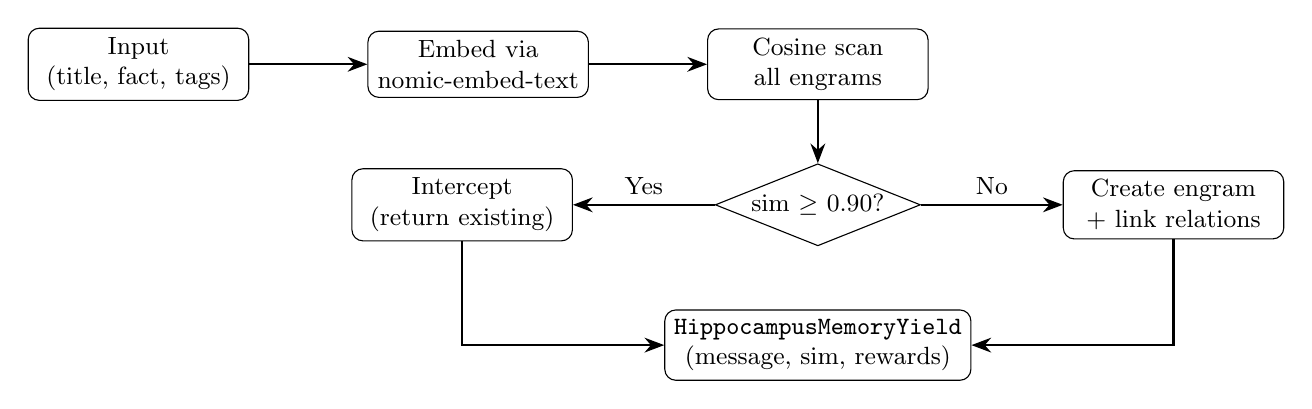
\begin{tikzpicture}[
  node distance=0.6cm and 1.5cm,
  box/.style={rectangle, draw, rounded corners, minimum width=2.8cm,
              minimum height=0.7cm, font=\small, align=center},
  decision/.style={diamond, draw, aspect=2.5, font=\small, align=center,
                   inner sep=1pt},
  arrow/.style={-{Stealth[length=2.5mm]}, thick}
]
  \node[box] (input) {Input\\(title, fact, tags)};
  \node[box, right=of input] (embed) {Embed via\\nomic-embed-text};
  \node[box, right=of embed] (cosine) {Cosine scan\\all engrams};
  \node[decision, below=0.8cm of cosine] (check) {sim $\geq$ 0.90?};
  \node[box, left=1.8cm of check] (reject) {Intercept\\(return existing)};
  \node[box, right=1.8cm of check] (create) {Create engram\\+ link relations};
  \node[box, below=0.8cm of check] (yield) {\texttt{HippocampusMemoryYield}\\(message, sim, rewards)};

  \draw[arrow] (input) -- (embed);
  \draw[arrow] (embed) -- (cosine);
  \draw[arrow] (cosine) -- (check);
  \draw[arrow] (check) -- node[above, font=\small] {Yes} (reject);
  \draw[arrow] (check) -- node[above, font=\small] {No} (create);
  \draw[arrow] (reject) |- (yield);
  \draw[arrow] (create) |- (yield);
\end{tikzpicture}
\end{center}

% ====================================================================
\section{Target Architecture: Typed Directed Hypergraph}
\label{sec:target}
% ====================================================================

\verified{} This section draws from the migration design document. The target architecture reconceptualizes
long-term memory as an exact hypergraph structure, replacing fuzzy vector
retrieval with deterministic algorithmic traversal.

% --------------------------------------------------------------------
\subsection{Core Hypergraph Definition}
% --------------------------------------------------------------------

\begin{definition}[Directed Hypergraph]
\label{def:hypergraph}
The new Hippocampus is modeled as a directed hypergraph:
\[
  H = (V, E)
\]
where:
\begin{itemize}[nosep]
  \item $V$ is a finite set of \textbf{vertices} representing discrete
    contextual system states.
  \item $E \subseteq \bigcup_{k \geq 2} V^k$ is a set of \textbf{directed
    hyperedges} representing relations or actions linking multiple elements.
\end{itemize}
\end{definition}

\begin{definition}[Ternary Engram Hyperedge]
\label{def:ternary}
An operational memory (engram) is modeled as a ternary relation (arity $k = 3$):
\[
  e_i = (v_{\text{state}}, \; v_{\text{action}}, \; v_{\text{next\_state}})
\]
where:
\begin{itemize}[nosep]
  \item $v_{\text{state}} \in V$ --- the system state at the time of memory formation.
  \item $v_{\text{action}} \in V$ --- the action or event that occurred.
  \item $v_{\text{next\_state}} \in V$ --- the resulting system state.
\end{itemize}
Higher-order contexts or temporal links correspond to increasing the arity of
the hyperedge beyond $k = 3$.
\end{definition}

\begin{remark}
This ternary structure $(s, a, s')$ is isomorphic to the standard
state--action--next-state transition tuple used in reinforcement learning.
The hypergraph formulation generalizes this by allowing a single hyperedge to
connect arbitrarily many vertices simultaneously.
\end{remark}

% --------------------------------------------------------------------
\subsection{Retrieval: Geodesic Traversal}
% --------------------------------------------------------------------

\verified{} Memory retrieval transitions from approximate nearest-neighbor
search to exact graph traversal:

\begin{definition}[Geodesic Distance]
\label{def:geodesic}
The distance between two vertices $v_s, v_t \in V$ is defined as the number
of hyperedges on the shortest path between them:
\[
  d_H(v_s, v_t) = \min \big\{ |P| : P \text{ is a path from } v_s
  \text{ to } v_t \text{ via hyperedges in } E \big\}
\]
This replaces cosine distance as the fundamental retrieval metric.
\end{definition}

\begin{pseudocodebox}[1: Memory Retrieval via Geodesic Traversal]
\label{alg:retrieve}
\begin{tabbing}
\textbf{proc} \= \textbf{RetrieveEngram}(current\_state, target\_goal): \\
\> $v_s \gets \text{FindNode}(\text{current\_state})$ \\
\> $v_t \gets \text{FindNode}(\text{target\_goal})$ \\
\> $P \gets \text{FindGeodesic}(H, v_s, v_t)$ \hfill\textit{\# Shortest path via hyperedges} \\
\> \textbf{return} $P$ \hfill\textit{\# Exact logical pathway} \\
\textbf{end proc}
\end{tabbing}
\end{pseudocodebox}

% --------------------------------------------------------------------
\subsection{Discrete Novelty and Graph-Theoretic Deduplication}
% --------------------------------------------------------------------

\verified{} The novelty computation must be redefined for the discrete setting:

\begin{definition}[Discrete Novelty]
\label{def:discrete-novelty}
When saving a new engram $e_{\text{new}}$, the system checks for isomorphic
sub-hypergraphs within $H$:
\begin{itemize}[nosep]
  \item If an exact isomorphic match exists: $\text{sim} = 1.0$ (intercept).
  \item Otherwise: $\text{sim}$ scales inversely with the
    \emph{graph edit distance} between $e_{\text{new}}$ and the nearest
    existing subgraph.
  \item Novelty scales by how much the new hyperedge increases the
    \emph{topological volume} of the local neighborhood.
\end{itemize}
\end{definition}

\begin{pseudocodebox}[2: Memory Addition via Hypergraph Rewriting]
\label{alg:add}
\begin{tabbing}
\textbf{proc} \= \textbf{AddEngram}(state, action, next\_state): \\
\> $v_c \gets \text{GetOrCreateNode}(\text{state})$ \\
\> $v_n \gets \text{GetOrCreateNode}(\text{next\_state})$ \\
\> $e_{\text{new}} \gets \text{CreateDirectedHyperedge}(v_c, \text{action}, v_n)$ \\
\> $\text{sim} \gets \text{CheckIsomorphism}(H, e_{\text{new}})$ \\
\> \textbf{if} $\text{sim} \geq 0.90$: \\
\> \textbf{return} Rejected \hfill\textit{\# Legacy intercept threshold preserved} \\
\> \textbf{end if} \\
\> $\text{RewriteGraph}(H, e_{\text{new}})$ \hfill\textit{\# Apply hypergraph rewrite rule} \\
\> $\text{CalculateAndGrantRewards}(\text{sim})$ \\
\textbf{end proc}
\end{tabbing}
\end{pseudocodebox}

% --------------------------------------------------------------------
\subsection{Neo4j Compatibility: Bipartite Reduction Middleware}
% --------------------------------------------------------------------

\verified{} A fundamental tension exists between the hypergraph formalism
(which requires $k$-ary relations) and Neo4j (which supports only binary
property-graph edges).

\begin{definition}[Bipartite Reduction]
\label{def:bipartite}
Each $k$-ary hyperedge $e \in E$ is projected into the Neo4j property graph
by representing it as a distinct \textbf{hyperedge node}, connected via binary
edges to its $k$ constituent element nodes:
\[
  e = (v_1, v_2, \ldots, v_k)
  \quad \xrightarrow{\text{project}} \quad
  n_e \text{ (hyperedge node)}, \;
  \{(n_e \to v_i)\}_{i=1}^{k}
\]
This standard bipartite reduction preserves the mathematical integrity of the
hypergraph while adhering to Neo4j's storage constraints.
\end{definition}

\begin{remark}
An alternative is to use NetworkX exclusively, which natively supports
arbitrary data structures and avoids the bipartite reduction overhead. The
trade-off is loss of Neo4j's production-grade persistence, indexing, and
query optimization.
\end{remark}

% --------------------------------------------------------------------
\subsection{Sleep Cycle Consolidation}
% --------------------------------------------------------------------

\verified{} The temporal lobe implements a cron-based ``Sleep State'' for
memory consolidation:

\begin{pseudocodebox}[3: Sleep Cycle Consolidation]
\label{alg:sleep}
\begin{tabbing}
\textbf{proc} \= \textbf{SleepStateConsolidation}(): \\
\> $\mathcal{E}_{\text{day}} \gets \text{GetDailyEngrams}(H)$ \\
\> \textbf{for} $e \in \mathcal{E}_{\text{day}}$: \\
\> $\Delta \gets \text{ExtractImprovements}(e)$ \hfill\textit{\# Identify consolidation targets} \\
\> \textbf{end for} \\
\> $\text{GenerateTrainingData}(\Delta)$ \\
\textbf{end proc}
\end{tabbing}
\end{pseudocodebox}

\noindent
\verified{} The Sleep State is located in \texttt{temporal\_lobe/inception.py}
and \texttt{tasks.py}. During low user activity, Talos suspends the frontal
lobe, processes the day's engrams, and uses \texttt{inception.py} to simulate
``dreams'' (sandboxed synthetic scenarios).

% --------------------------------------------------------------------
\subsection{Planned Module Architecture}
% --------------------------------------------------------------------

\verified{} The migration document specifies three new core modules:

\begin{table}[h]
\centering
\begin{tabular}{@{}lp{9cm}@{}}
\toprule
\textbf{Module} & \textbf{Responsibility} \\
\midrule
\texttt{HypergraphMemoryManager} &
  Manages the bipartite Neo4j or NetworkX mapping. Handles vertex
  creation, hyperedge construction, and graph queries. \\[0.5em]
\texttt{EngramRewriter} &
  Implements hypergraph rewriting rules. The hypergraph evolves by
  transforming discrete collections of relations at each timestep. \\[0.5em]
\texttt{SleepConsolidator} &
  Generates synthetic \texttt{IterationDefinitions} during the sleep
  cycle. Implemented within \texttt{inception.py}. \\
\bottomrule
\end{tabular}
\caption{New core modules for the hypergraph Hippocampus.}
\label{tab:new-modules}
\end{table}

% ====================================================================
\section{The Continuous--Discrete Bridge}
\label{sec:bridge}
% ====================================================================

\verified{} The central unresolved tension in the migration is the mapping from
continuous $\mathbb{R}^{768}$ embeddings to discrete hypergraph vertices:

\begin{quote}
\itshape
``The exact mapping from $\mathbb{R}^{768}$ continuous embeddings to discrete
hypergraph vertices remains an open question.''
\end{quote}

\noindent
\verified{} Four resolution approaches have been proposed:

\begin{enumerate}[label=\textbf{\arabic*.}, leftmargin=2em]
  \item \textbf{Hybrid Nodes} --- Each vertex carries both a discrete UUID
    (for graph traversal) and a compressed vector (for fuzzy recall as
    fallback).

  \item \textbf{Product Quantization} --- FAISS-based $8$--$32\times$
    compression of the embedding vectors, preserving approximate similarity
    while reducing the continuous space to a manageable finite codebook.

  \item \textbf{Learned Discretization (VQ-VAE)} --- Train a codebook via
    Vector Quantized Variational Autoencoder:
    \[
      \text{encoder} : \mathbb{R}^{768} \longrightarrow \{0, 1, \ldots, 4095\}
    \]
    Each engram is represented by its codebook index rather than its full
    embedding vector.

  \item \textbf{Hierarchical Decomposition} --- Three nested levels:
    \begin{itemize}[nosep]
      \item Level~1: Discrete state nodes (vertices in $V$)
      \item Level~2: Vector embeddings (auxiliary cached views)
      \item Level~3: Hyperedge relations (edges in $E$)
    \end{itemize}
\end{enumerate}

\begin{openquestion}
Which discretization strategy best preserves retrieval fidelity while enabling
deterministic graph traversal? The VQ-VAE approach aligns well, but requires a
sufficiently large and well-structured training corpus of engrams.
\end{openquestion}

% ====================================================================
\section{Migration Strategy}
\label{sec:migration}
% ====================================================================

\verified{} The migration from pgvector to hypergraph proceeds in four phases:

\begin{enumerate}[label=\textbf{Phase \arabic*:}, leftmargin=3.5em]
  \item \textbf{Infrastructure} --- Deploy Neo4j (or initialize NetworkX
    in-process) alongside existing PostgreSQL and Redis.

  \item \textbf{Dual-Write} --- \texttt{mcp\_engram\_save} writes to both
    pgvector (semantic vectors) and the hypergraph (rewrite rule insertions).
    Both stores are kept in sync.

  \item \textbf{Cut-Over} --- Point \texttt{mcp\_engram\_read} and
    \texttt{mcp\_engram\_search} to hypergraph geodesic traversal endpoints.
    pgvector becomes read-only fallback.

  \item \textbf{Consolidation} --- Enable \texttt{inception.py} to process
    graph engrams during the sleep cycle. Full system operates on hypergraph
    as primary substrate.
\end{enumerate}

\subsection{Legacy Data Migration}

\verified{} Existing 768-dimensional vectors are instantiated as disconnected
vertices in the new hypergraph. A batch process constructs edges by evaluating
cosine similarities as semantic links, bootstrapping the initial graph topology
from the continuous metric.

\subsection{Rollback Strategy}

\verified{} The legacy pgvector repository is maintained as a read-only
fallback. If hypergraph retrieval fails or produces degenerate paths, the
system gracefully degrades to nearest-neighbor vector search.

\newpage

% ====================================================================
\section{Architectural Delta Summary}
\label{sec:delta}
% ====================================================================

\begin{table}[h]
	\centering
	\begin{tabular}{@{}p{4cm}p{5cm}p{5cm}@{}}
		\toprule
		\textbf{Aspect} & \textbf{Current (pgvector)} & \textbf{Target (Hypergraph)} \\
		\midrule
		Storage backend &
		PostgreSQL + pgvector &
		Neo4j or NetworkX + PostgreSQL (fallback) \\[0.5em]
		Memory unit &
		768-dim vector + metadata &
		Ternary hyperedge $(s, a, s')$ \\[0.5em]
		Retrieval metric &
		Cosine similarity &
		Geodesic distance (shortest path) \\[0.5em]
		Novelty computation &
		$\max(0, 1 - \text{sim})$ &
		Isomorphism check + graph edit distance \\[0.5em]
		Deduplication &
		Cosine threshold $\geq 0.90$ &
		Subgraph isomorphism detection \\[0.5em]
		Consolidation &
		Not yet implemented &
		Sleep cycle via \texttt{inception.py} \\[0.5em]
		Self-improvement &
		Weight Updates &
		Weight Updates + Future Structural Rewriting \\[0.5em]
		Formal substrate &
		$\mathbb{R}^{768}$ vector space &
		Three-layered Hypergraph Substrate\\
		\bottomrule
	\end{tabular}
	\caption{Architectural delta: current vs.\ target Hippocampus.}
	\label{tab:delta}
\end{table}

\newpage

% ====================================================================
\section{Open Questions and Future Work}
\label{sec:open}
% ====================================================================

\begin{openquestion}
\textbf{Discretization strategy selection.} Which of the four proposed
approaches (Hybrid Nodes, Product Quantization, VQ-VAE, Hierarchical
Decomposition) should be implemented? The current architectural preference
is for VQ-VAE with end-to-end training, storing codebook indices rather than
raw vectors. \speculative{}
\end{openquestion}

\begin{openquestion}
\textbf{Intercept threshold adaptation.} The fixed $0.90$ cosine threshold
works for continuous embeddings but may need recalibration for discrete
graph-theoretic novelty. Should the threshold be adaptive, learned, or
replaced by a structural criterion (e.g., subgraph diameter)? \speculative{}
\end{openquestion}

% ====================================================================
\section{References}
\label{sec:references}
% ====================================================================

\begin{enumerate}[label={[\arabic*]}, leftmargin=2.5em, nosep]
  \item \textbf{Talos Codebase} --- \texttt{hippocampus/models.py},
    \texttt{hippocampus/hippocampus.py}, \texttt{common/models.py}.
    Production source code. \verified{}

  \item \textbf{Hippocampus Documentation} ---
    \texttt{docs/doc-generator\_talos-only/hippocampus\_\_documentation.md}.
    Auto-generated module documentation with mathematical appendix. \verified{}

  \item \textbf{LIVE\_CODEBASE\_ANALYSIS.md} ---
    \texttt{docs/LIVE\_CODEBASE\_ANALYSIS.md}.
    System-wide analysis including memory system section. \verified{}


  \item \textbf{Hippocampus Memory Migration to Hypergraphs} ---
    \texttt{docs/final\_docs/are-self\_hippocmpus\_memory\_migration-to-hypergraphs.pdf}.
    Migration design document with algorithms and data model. \verified{}


  \item \textbf{are-self Whitepaper} ---
    \texttt{docs/are\_self\_whitepaper.tex}.
    System design overview and formal definitions. \verified{}

  \item \textbf{are-self Preprint Article} ---
    \texttt{docs/final\_docs/are-self\_preprint\_article.pdf}.
    Brain-themed modular decomposition. \verified{}

  \item C.~Berge, \textit{Graphs and Hypergraphs}, North-Holland, 1973.

  \item A.~Bretto, \textit{Hypergraph Theory: An Introduction},
    Springer, 2013.

  \item Y.~Feng et al., ``Hypergraph Neural Networks,''
    \textit{Proc.\ AAAI}, 2019.
\end{enumerate}

\end{document}
